\section{Experimental Results}\label{sec:benchmarks}

\subsection{Goals}

In our preliminary experiments with the running BigchainDB end-to-end, we found that the biggest limiter of performance was in how the database itself (RethinkDB) interacted with the physical compute resources (write speed, IO among nodes).
This was not surprising, because the BigchainDB’s design was about “getting out of the way” of what the database itself is good at.

Therefore, we could frame the experiments around performance testing of RethinkDB.
The goal was to test scalability properties, understand its limits and see if we could reach a speed of $1$M transactions per second.

Full benchmarks on the performance of BigchainDB will appear in the near future.

\subsection{Experiments on Throughput}

The setup for the following experiments is described in detail in Appendix \ref{subsec:benchmarks_setup}.

In one experiment, we increased the number of nodes every ten seconds, up to $32$ nodes.
We used RethinkDB's System Statistics Table to record the write throughput over time.

\begin{figure}[!ht]
  \centering
  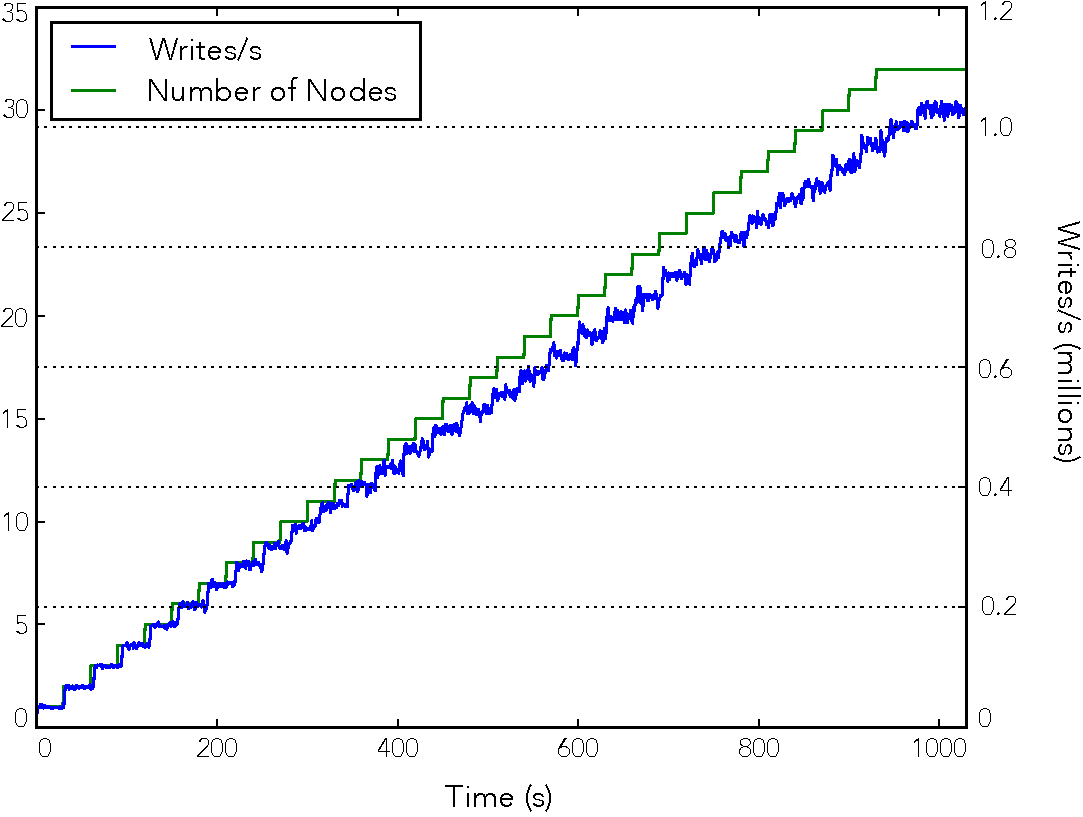
\includegraphics[width=0.7\textwidth]{figure_14.pdf}
  \caption{Time-series plot, where when we increased the number of nodes, the throughput in terms of writes/s increased accordingly.}
  \label{fig:bigchain_throughput_vs_nodes}
\end{figure}

Figure \ref{fig:bigchain_throughput_vs_nodes} shows how write throughput increased every time a node was added.
When the number of nodes reached $32$, the write throughput was just over $1$ million writes per second (i.e. $1000$ blocks per second, with $1000$ transactions per block).

\begin{figure}[!ht]
  \centering
  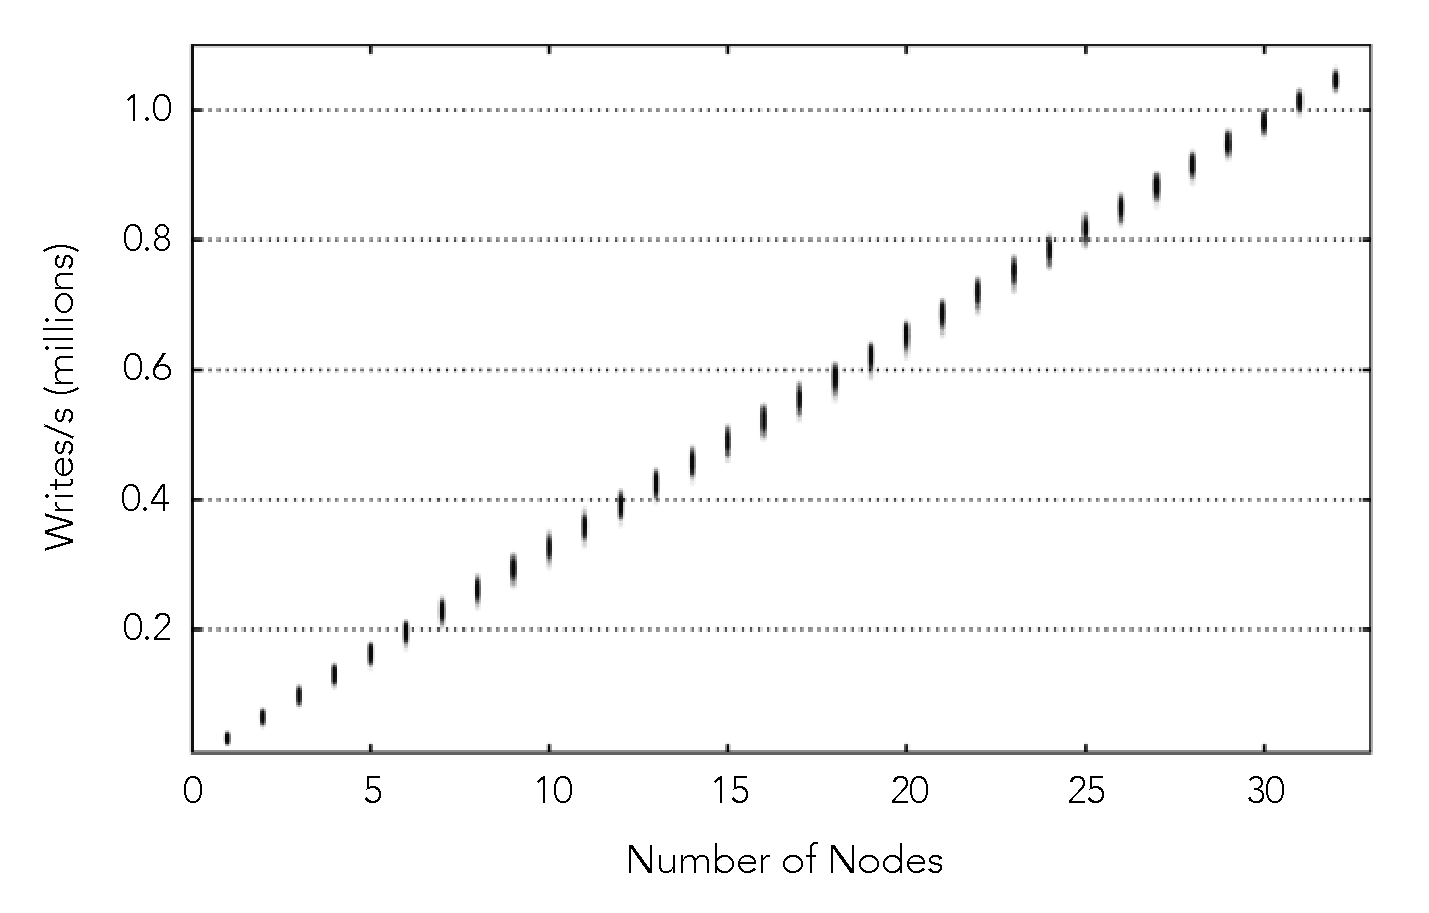
\includegraphics[width=0.7\textwidth]{figure_15.pdf}
  \caption{Writes/s versus number of nodes. There is linear scaling in write performance with the number of nodes. With $32$ nodes, we can achieve over a million writes/s.}
  \label{fig:bigchain_writes_vs_nodes}
\end{figure}

Figure \ref{fig:bigchain_writes_vs_nodes} shows data from the same experiment, except it shows how write throughput was affected by the number of nodes (rather than time).
The plot is both boring and exciting: it shows how write throughput increases linearly with the number of nodes.
$32$ nodes gives performance of $>1,000,000$ writes/s.

\subsection{Other Experiments}
The appendix \ref{appendix:benchmarks} contains descriptions of further experiments.